%-----------------------------------------------%
% Início do plano de aula
%-----------------------------------------------%
\thispagestyle{empty}
\begin{center}
	\begin{minipage}[!]{\linewidth}
        \begin{minipage}[!]{.19\linewidth}
            
\includegraphics[width=\linewidth]{img/logo.png}           
        \end{minipage}
        \begin{minipage}[!]{.8\linewidth}
            \center
            \ABNTEXchapterfont\normalsize\MakeUppercase{\imprimirinstituicao}
            \par
            \vspace*{10pt}                     
            \ABNTEXchapterfont\normalsize\MakeUppercase{\centro}
            \par
            \vspace*{10pt}           
            \ABNTEXchapterfont\normalsize\MakeUppercase{\disciplina}
        \end{minipage}        
    \end{minipage}
    \\ \vspace{0.5cm}
    \rule{\textwidth}{.5pt}   
\end{center}
    \textual
    \begin{center}
      \section{Ondas I}
      \par
    \end{center}
    
    \noindent \textbf{Estagiário(a): }\imprimirautor 
    
    \noindent \textbf{U.E.: }EEB Giovani Pasqualini Faraco
    
    \noindent \textbf{Série: }2º Ano\hfill{}\textbf{Turma: }2º--5
    
    \noindent \textbf{Aula:} 003\hfill{}\textbf{Data:} XX/XX/2022\hfill{}\textbf{Duração:} $45\min$
    \rule{\textwidth}{.5pt}
    \bigskip{}  
    

    \noindent
    \begin{center}
      \textbf{Ondas: Grandezas Descritivas}
    \par\end{center}

    \noindent \textbf{Resumo da aula:} Será introduzido o conceito de ondas de forma a dar suporte ao estudo da propagação luminosa.

    \par\noindent \textbf{Habilidades BNCC: }EF09CI06; EF09CI04.
    \vspace*{20pt}
    
    \subsection*{Objetivo de Aprendizagem}
    \begin{itemize}
        \item Compreender os fundamentos do modelo ondulatório e suas principais características;
        \item Diferenciar o modelo ondulatório do modelo corpuscular;
        \item Conhecer os diferentes tipos de ondas e suas principais características;
        \item Calcular a velocidade de uma onda qualquer com base em suas grandezas constituintes.
    \end{itemize}
    \medskip{}
    %\vfill    
    \noindent \textbf{Núcleo Conceitual:} \emph{Teoria ondulatória; Teoria corpuscular; Conceitos básicos inerentes à ondulatória.}

    %\newpage
    \section*{Procedimento Didático} 
    \noindent \emph{1º Momento:} Como medir a velocidade de uma onda?
	\par\noindent\rule{.3\textwidth}{.5pt}  
    \par\noindent \textbf{Tempo previsto:} 15 minutos  

    \noindent \textbf{Dinâmica:} Retomar as discussões da última aula, relembrando as principais observações obtidas pela análise das simulações do \emph{Phet}, conforme ilustra a \autoref{fig:phet-a} a seguir:
    \vspace*{10pt}
    \begin{figure}[!ht]        
        \centering              
        \subfloat[\label{fig:phet-1}]{
            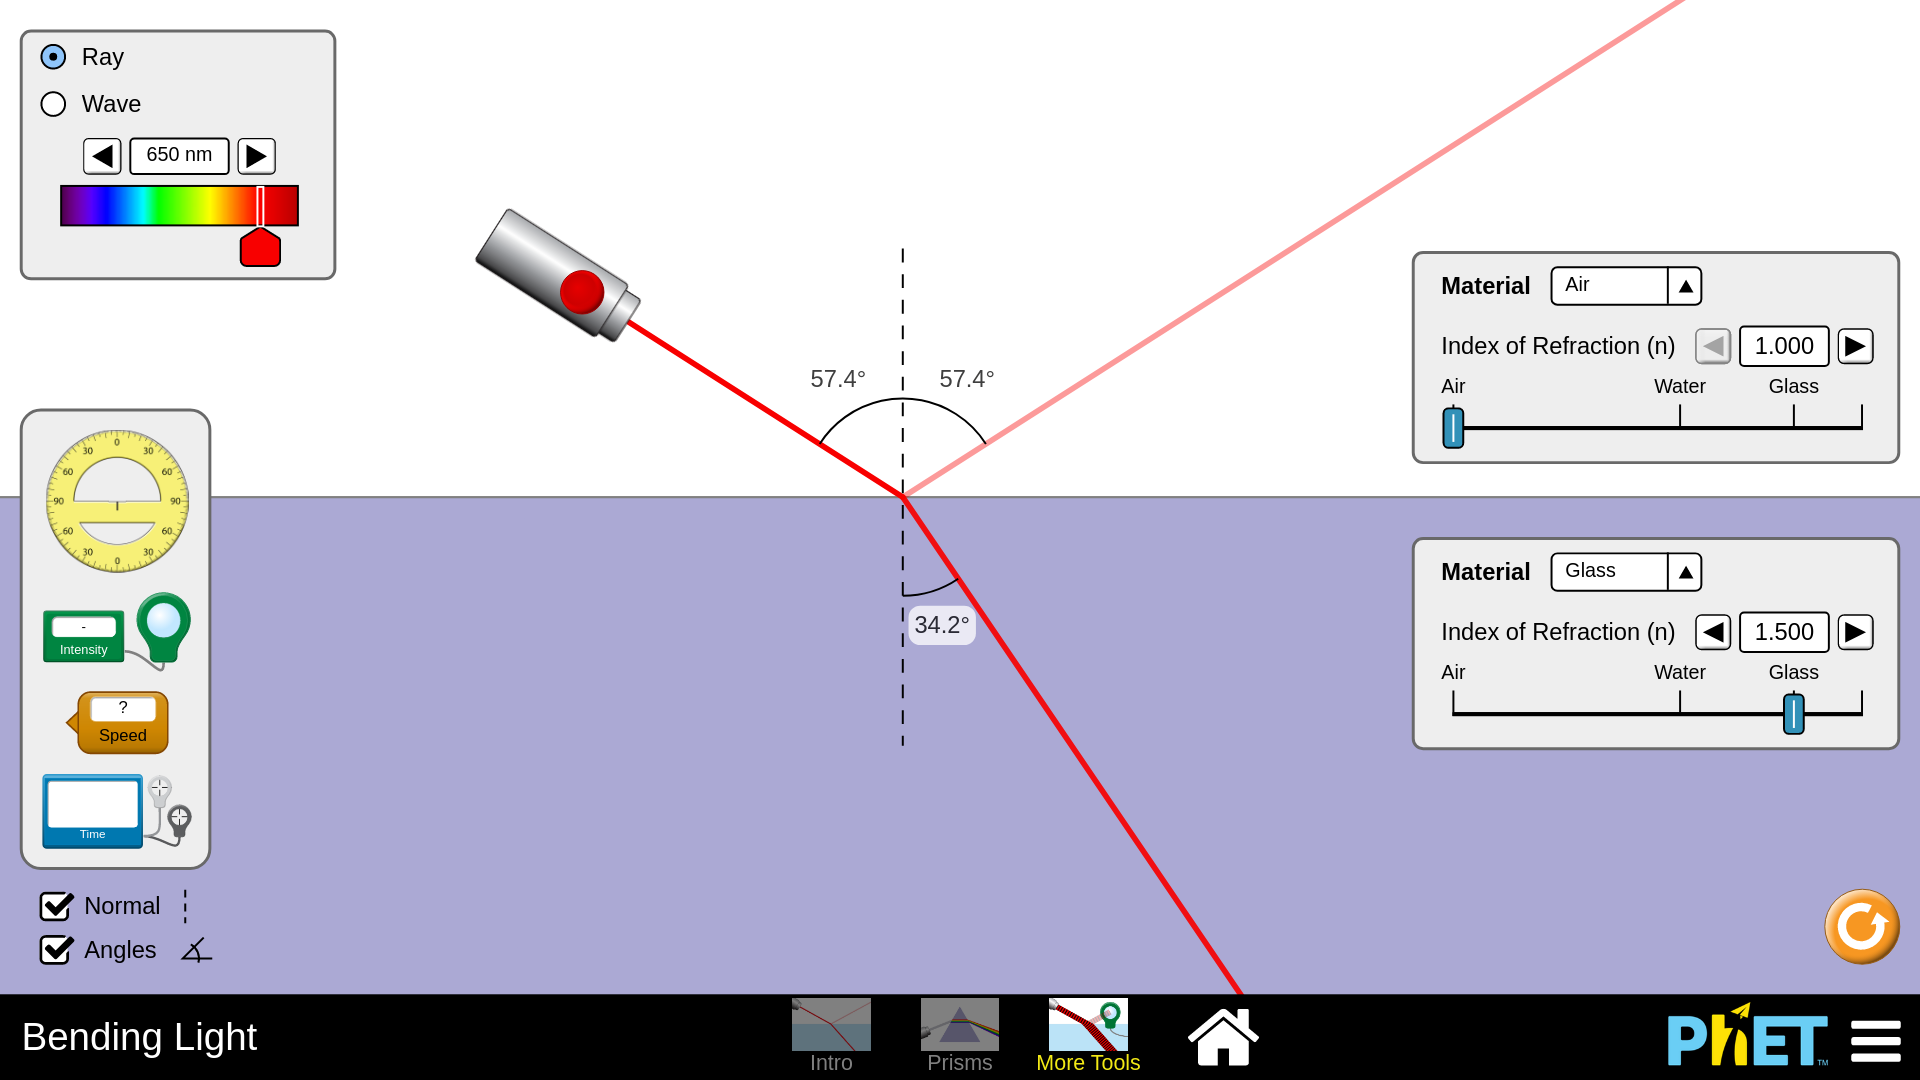
\includegraphics[width=.45\textwidth]{img/phet-1.png}
        }\hfill
        \subfloat[\label{fig:phet-2}]{
            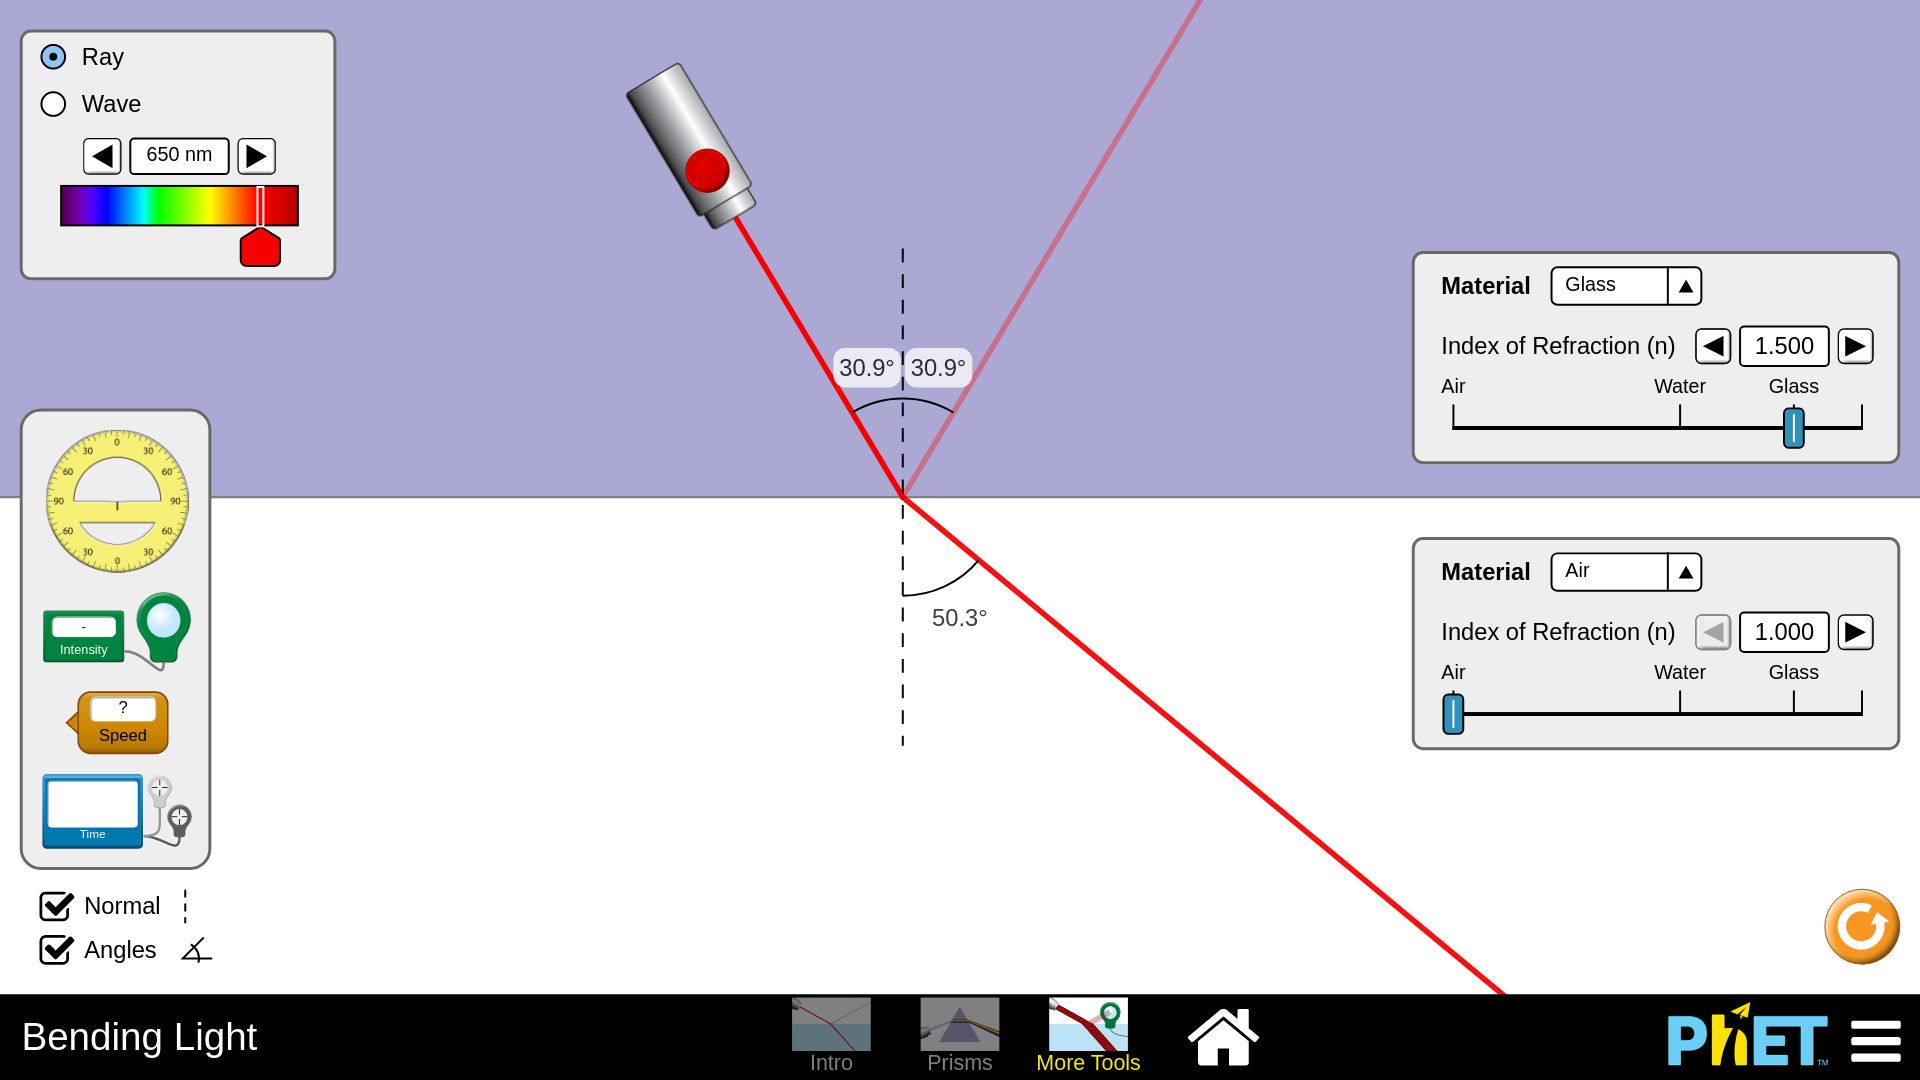
\includegraphics[width=.45\textwidth]{img/phet-2.png}
        }        
        \caption{Simulação \emph{Phet} em (a), feixe luminoso partindo do ar para o vidro, raio refratado aproxima-se da normal ao ponto de contato e em (b), feixe luminoso partindo do vidro para o ar, raio refratado afasta-se da normal ao ponto de contato.}
        \label{fig:phet-a}
    \end{figure}
    \vspace*{10pt}
    \par \noindent Destacar que para ambos os casos vistos, o ângulo refletido tem o mesmo valor que o ângulo incidente e que se os meios são idênticos, o raio simplesmente atravessa como se não houvesse meio algum.
    
    \par\noindent\textbf{Discussão:} Vocês identificaram que os desvios que a luz sofre, na transição entre os meios diferentes, é decorrente de uma mudança na velocidade de propagação do feixe luminoso, agora:
    \begin{itemize}
        \item Em qual situação a velocidade da luz é maior ou menor?
        \item Como calcular a velocidade da luz nestes casos?
        \item Do que vocês conhecem a respeito do conceito de velocidade até agora visto, o que é necessário para que algo altere a sua velocidade?
        \item De que forma podemos utilizar estas ideias (cinemática, dinâmica e etc) aqui (ondas)?
    \end{itemize}

    Não é possível prever o que o professor obterá como respostas para estas questões, de qualquer forma, o professor deve encaminhar a discussão para as diferenças de tratar destes conceitos em ambos os modelos.

    \vspace{50pt}
    \noindent \emph{2º Momento:} Construindo um modelo ondulatório para a luz
	\par\noindent\rule{.3\textwidth}{.5pt}    
    \par\noindent \textbf{Tempo previsto: }20 minutos
	

    \noindent \textbf{Dinâmica:} Mencionar que há duas formas (modelos) de responder às questões levantadas anteriormente e que isso gerou muita discussão entre os séculos XII e XIII, sobre em qual dos modelos deve-se atribuir os fenômenos ópticos. A seguir, o professor deve apresentar os modelos como segue:

    \begin{itemize}
        \item \emph{Modelo corpuscular newtoniano}, a luz era composta por minúsculas partículas, fenômenos como reflexão e refração eram explicados com base na teoria mecanicista de Newton, tinha o próprio Newton como seu principal defensor\footnote{Não há consenso entre os historiadores da ciência, de que Newton defendeu veementemente um modelo em detrimento do outro, como apontam as pesquisas \cite{FELIPHE:2019,FABIO:2009,YOUNG:1801}.}. Prevê uma velocidade de propagação maior para a luz em meios mais densos, como a água por exemplo, do que nos meios menos densos, esta tese é suportada pelo seguinte argumento \cite{PEDUZZI:2022}:
        
        \begin{citacao}
            Como o raio de luz se aproxima da normal, na passagem da luz do ar para a água, a hipótese corpuscular sugeria que seria necessária a existência de uma força atuando no sentido de acelerar o corpúsculo para dentro da água, aumentando, por conseguinte, sua velocidade. 
        \end{citacao}
        
        \item \emph{Modelo ondulatório}, a luz é concebida como uma onda, fenômenos como reflexão e refração são explicados pela Lei de Snell-Descartes, tem como principais defensores, Huygens, Young, Hooke dentre outros. Prevê uma velocidade de propagação para a luz menor para a água do que para o ar, segundo \cite{PEDUZZI:2022} a argumentação dos que defende o modelo ondulatório é de que:
        
        \begin{citacao}
            \ldots tendo em vista que o raio de luz refratado aproximam-se da normal em meios mais densos, decorre disto que o comprimento da onda da luz refratada sofre redução. Se a frequência é constante e só depende das características da fonte luminosa geradora do feixe, a velocidade da luz deve portanto diminuir.
        \end{citacao}
    \end{itemize}

    Ressaltar que o modelo corpuscular foi predominante durante aproximadamente 200 anos em virtude do prestígio de Newton, e que só foi começar a entrar em derrocada a partir dos experimentos de Young (dupla fenda) no século XIX, tornando-se amplamente aceito somente a partir do século passado.

    Após a apresentação das bases históricas, apresentar o modelo ondulatório de forma geral, a partir dos seguintes conceitos e conforme detalhado na \autoref{sec:nocoes-basicas-ondas}:

    \begin{itemize}
        \item Caracterização de ondas;
        \item Classificação de ondas;
        \item Grandezas oscilatórias;
        \begin{itemize}
            \item Comprimento de onda;
            \item Período;
            \item Frequência;
            \item Velocidade.
        \end{itemize}
    \end{itemize}   
    

	\vspace{50pt}
    \noindent \emph{3º Momento:} Estimando a velocidade de ondas já conhecidas.
	\par\noindent\rule{.3\textwidth}{.5pt}      
    \par\noindent \textbf{Tempo previsto: }10 minutos
    \par\noindent \textbf{Dinâmica:} Após estabelecida a equação da velocidade de uma onda, pedir que diferentes grupos de alunos estimem a velocidade das ondas do espectro visível a partir dos dados da \autoref{tab:alguns-espectros-do-visivel}:
    \vspace*{10pt}

    \begin{table}[!ht]
        \centering
        \begin{tabular}{|c|c|c|}
        \hline
        \textbf{Cor}      & \textbf{$\lambda(\textrm{nm})$} & \textbf{Frequência $f(10^{12}\textrm{Hz})$} \\ \hline
        \textbf{Vermelho} & 625                             & 480                                         \\ \hline
        \textbf{Laranja}  & 590                             & 510                                         \\ \hline
        \textbf{Amarelo}  & 565                             & 530                                         \\ \hline
        \textbf{Verde}    & 500                             & 600                                         \\ \hline
        \end{tabular}
        \caption{Comprimentos de onda $\lambda$ e frequências $f$ de algumas faixas de valores do espectro visível.}
        \label{tab:alguns-espectros-do-visivel}
    \end{table}
    \vspace*{10pt}

    \noindent Todos devem encontrar valores muito próximos a $2,99\times 10^8\mps$. Questionar o motivo pelo qual todos encontraram valores muito próximos, e se já conhecem este valor de velocidade. Relacionar esta velocidade com a velocidade da luz no vácuo e justificar que pelo fato do ar, ser o meio material cujo o qual oferece a menor resistência à passagem da luz, os físicos normalmente utilizam velocidade da luz no ar igual à velocidade da luz no vácuo.
    \newpage
    Análogo ao que foi feito pra velocidade da luz, sugerir que a partir da \autoref{tab:notas-musicais} logo a abaixo estimem a velocidade do som
    \vspace*{10pt}
    
    \begin{table}[!ht]
        \centering
        \begin{tabular}{|c|c|c|}
        \hline
        \textbf{Nota} & \textbf{$\lambda(\textrm{m})$} & \textbf{Frequência $f(\textrm{Hz})$} \\ \hline
        \textbf{C}    & 21,04                          & 16,35                                \\ \hline
        \textbf{D}    & 18,74                          & 18,35                                \\ \hline
        \textbf{E}    & 16,70                          & 20,60                                \\ \hline
        \textbf{F}    & 15,76                          & 21,82                                \\ \hline
        \textbf{G}    & 14,04                          & 24,50                                \\ \hline
        \textbf{A}    & 12,51                          & 27,50                                \\ \hline
        \textbf{B}    & 11,14                          & 30,86                                \\ \hline
        \end{tabular}
        \caption{Comprimentos de onda $lambda$ e frequências $f$ de algumas notas musicais.}
        \label{tab:notas-musicais}
    \end{table}
    \vspace*{10pt}
    
    Dedicar o restante da aula para discussão destes resultados e tiragem de dúvidas sobre a exposição.